%%%%%%%%%%%%%%%%%%%%%%%%%%%%%%%%%%%%%%%%%%%%%%%%%%%%%%%%%%%%%%%%%%%%%%%%
% TFG: Vigilancia Tecnológica y Minería de Opiniones en RRSS
% Escuela Técnica Superior de Ingenierías Informática y de Telecomunicación
% Realizado por: Miguel Keane Cañizares
% Contacto: miguekeca@correo.ugr.es 
%%%%%%%%%%%%%%%%%%%%%%%%%%%%%%%%%%%%%%%%%%%%%%%%%%%%%%%%%%%%%%%%%%%%%%%%

\chapter{Análisis y Planificación}

El proyecto constará de varias fases importantes a tener en cuenta, de las cuales distinguiremos de forma importante cuatro. Preparación, Desarrollo, Obtención de Información y análisis de resultados. 

\subsection{Preparación}

Esta fase será tiempo dedicado principalmente al estudio del lenguaje de programación Python, aprender cuales son sus diferentes librerías y cómo aplicar los conocimientos de programación obtenidos durante el grado en este lenguaje el cual es la primera vez que utilizo. Además será necesario conocer como funciona la API de Twitter y la API de MeaningCloud, para poder obtener la información y luego analizarla. Repasar como funciona una base de datos MongoDB, utilizada previamente durante los años lectivos, pero en necesidad de refrescar los conocimientos. 

También ha sido elegida LaTex para el desarrollo de la memoria, cuyos parámetros también habrán de ser estudiados para la correcta realización del proyecto junto con Excel y sus diferentes funciones, para poder sacar el máximo partido al proyecto. 

Es importante también notar que para el proyecto se requerirá de acceso a dos APIs distintas, por lo que es necesario registrarse en Twitter Dev para obtener las claves de Twitter y en la plataforma de MeaningCloud, para poder hacer uso de su análisis con la clave que proporcionan.

Finalmente, se ha optado por la realización de un diagrama de Gantt para hacer un correcto seguimiento del proyecto. 

\subsection{Desarrollo}

En esta fase será para hacer el desarrollo software correspondiente, crear los scripts que sean necesarios para obtener la información, para llevarla a analizar y para procesarla, todo mientras la información obtenida como los resultados de los análisis se almacene correctamente. 

\subsection{Obtención de información}

Una vez desarrollados los primeros scripts, haré uso de los métodos la API de stream para escuchar en directo con la palabra o palabras claves deseadas. Este proceso podrá ser largo y controlado, para obtener una cantidad de información aceptable para el análisis y almacenar la misma en su respectiva base de datos MongoDB. 

\subsection{Análisis de resultados}

Cuando ya disponemos de la información deseada, desde la propia base de datos MongoDB enviaremos la información a la API de MeaningCloud. La cual será procesada y la respuesta la almacenaremos doblemente, en una base de datos MongoDB por si requerimos de analizarla de nuevo y en un fichero CSV, el cual es ideal para luego poder analizar los resultados. Además en esta fase se desarrollará un script que pueda crear nubes con las palabras más utilizadas en la información descargada. También se tratará de obtener conclusiones sobre los datos obtenidos que puedan ser prácticas para una empresa. 
Es importante notar que en la versión gratuita de MeaningCloud solo tendremos 20000 créditos para gastar. Por cada tweet, debido a su longitud se gastará un crédito por tweet analizado. 




%	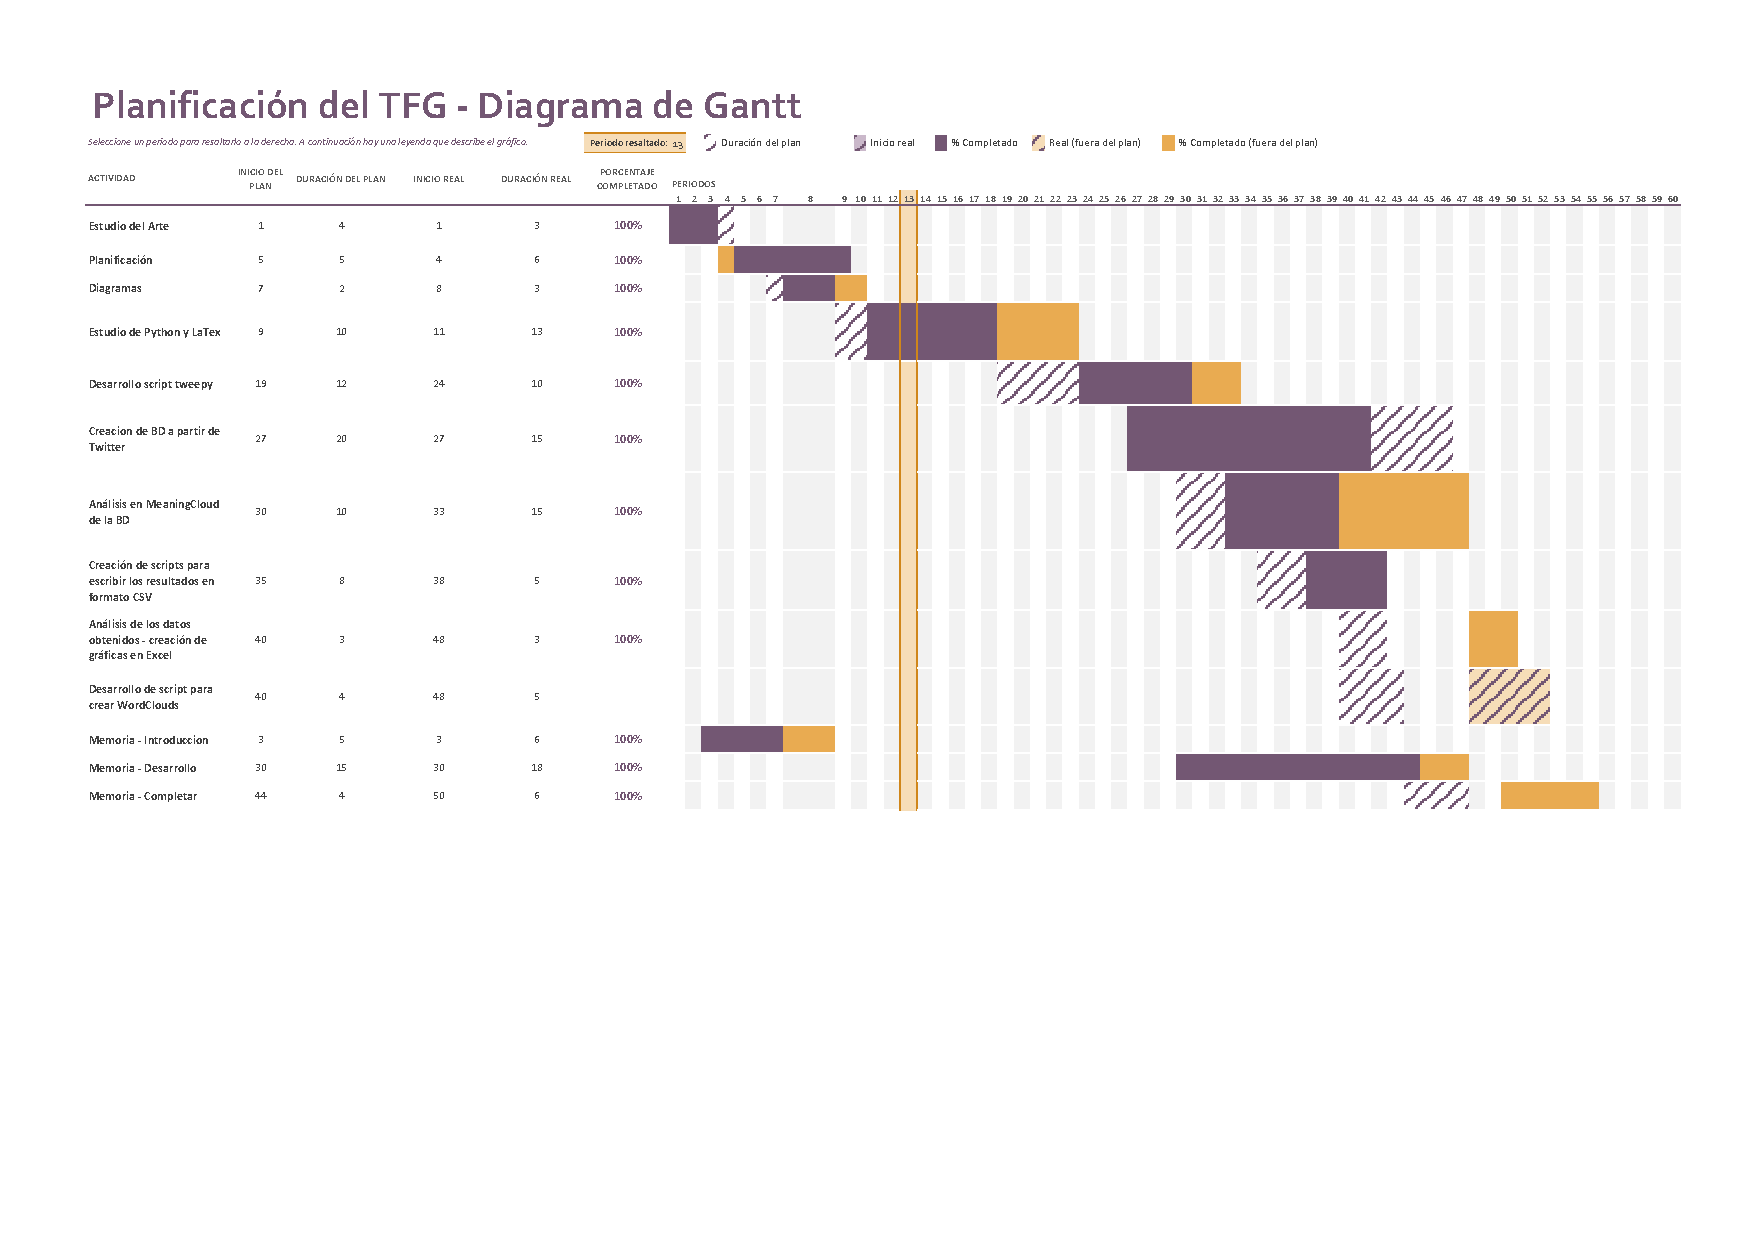
\includepdf[pages={1}]{capitulos/Gantt1-wordcloud.pdf}

\begin{figure}[h]
	\centering
	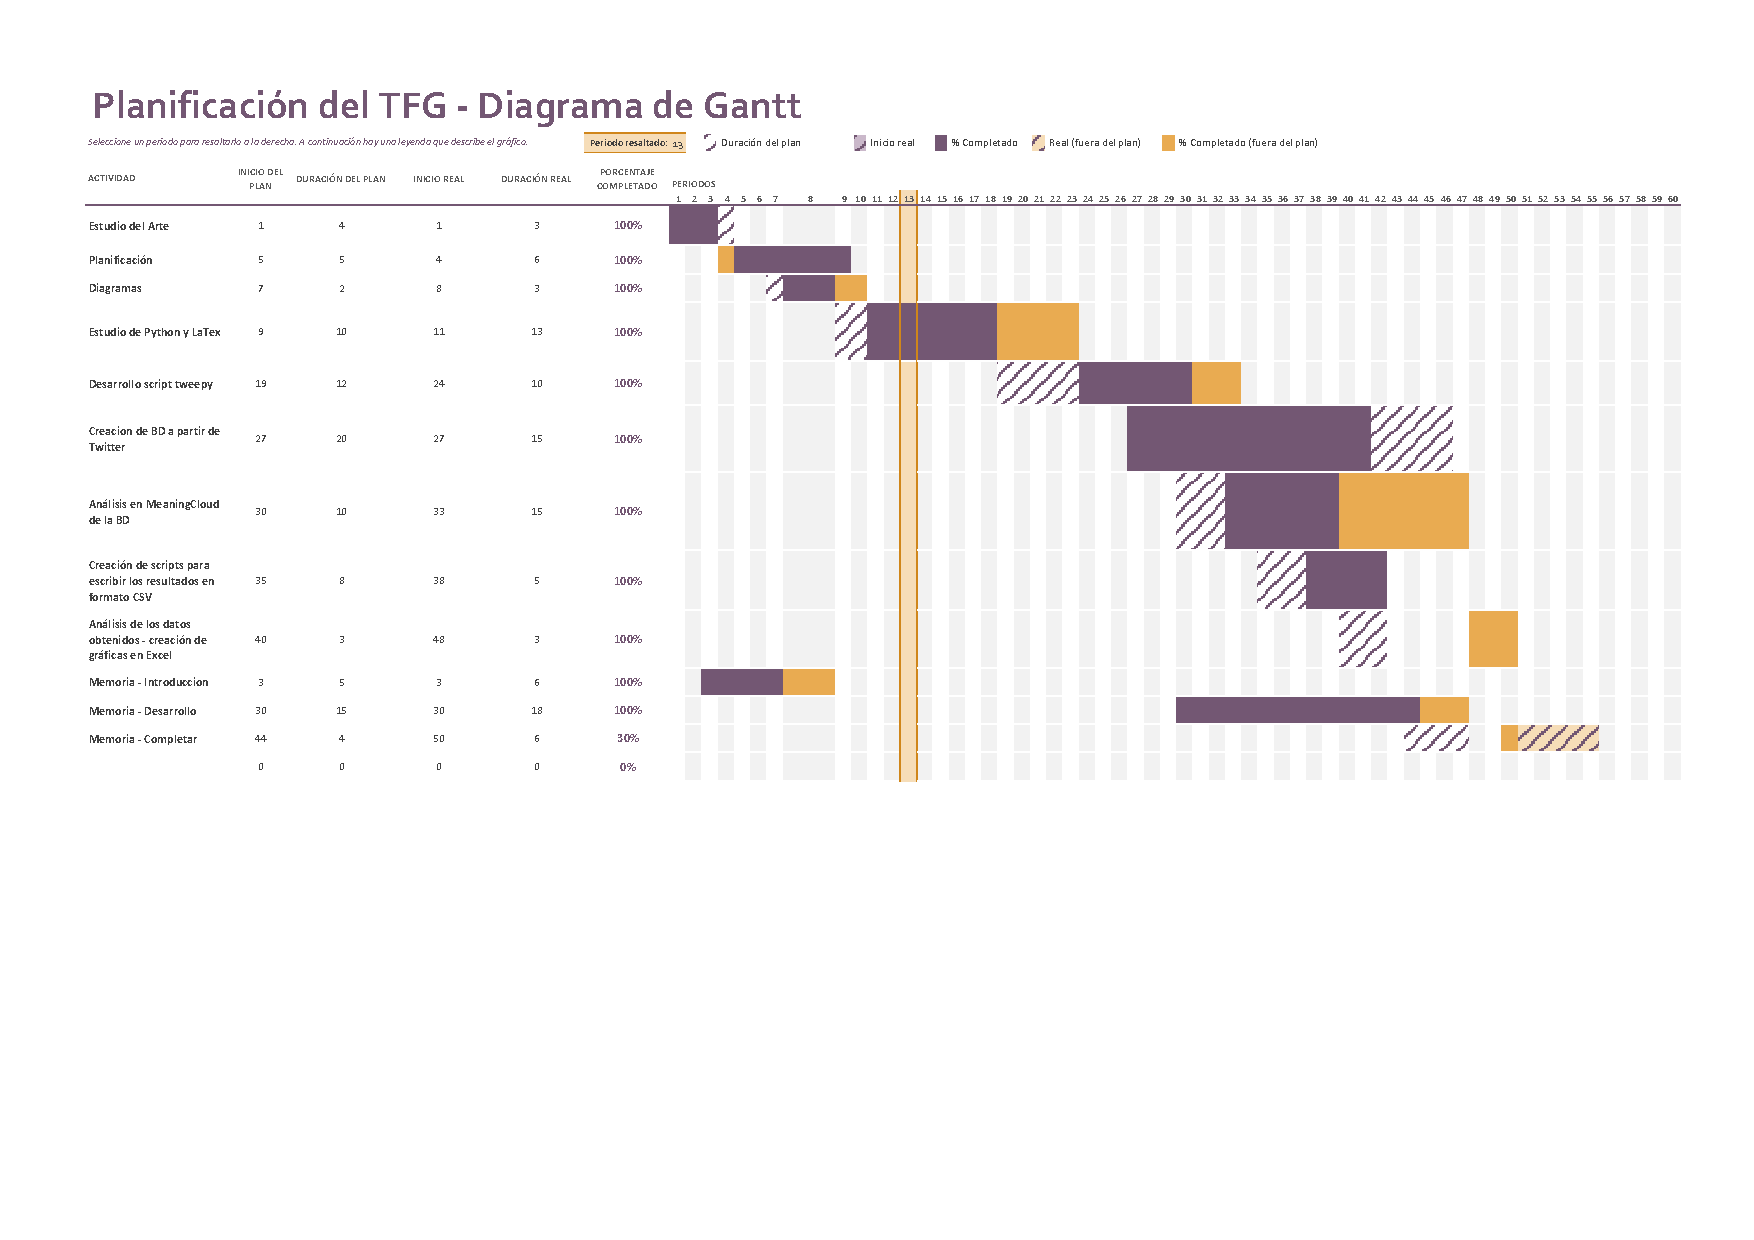
\includegraphics[scale=.6]{capitulos/Gantt1.pdf}
	\caption{Diagrama de Gantt}
	\label{fig:gantt}
\end{figure}
















